\documentclass[conference]{IEEEtran}
\IEEEoverridecommandlockouts
\usepackage{cite}
\usepackage{amsmath,amssymb,amsfonts}
\usepackage{algorithmic}
\usepackage{graphicx}
\usepackage{textcomp}
\usepackage{xcolor}
\usepackage{float}
\def\BibTeX{{\rm B\kern-.05em{\sc i\kern-.025em b}\kern-.08em
    T\kern-.1667em\lower.7ex\hbox{E}\kern-.125emX}}
\begin{document}

\title{A comparison of multidisciplinary research in Mexico, USA, China, UK, Germany, and Japan \\
}

\author{\IEEEauthorblockN{Farid Jacome Velasco}
\IEEEauthorblockA{\textit{School of Engineering and Science} \\
\textit{Tecnologico de Monterrey}\\
Ciudad de México, Mexico \\
A01654534@tec.mx}
\and
\IEEEauthorblockN{José Eduardo Zárate Aranda}
\IEEEauthorblockA{\textit{School of Engineering and Science} \\
\textit{Tecncologico de Monterrey}\\
Guadalajara, Mexico \\
A01630299@tec.mx}
}

\maketitle
%---------------------------------------------------------------------------------------------------------------
\begin{abstract}
Academic productivity and excellence are part of the knowledge factor that impacts a country's economy. Currently, land, capital, and work are no longer the only ones determining the country's productivity. Scientific knowledge is the driving force for the development of a society and impacts the life quality of a nation's citizens. Therefore, it is essential to analyze the current scenario of Mexico in terms of academic productivity and excellence compared with the top countries in this factor. One of the current tendencies is the multidisciplinary research teams to improve the generation of innovative value in the pool of knowledge. Given that fact, the multidisciplinary published articles, the citation counts, the relevant topics, and the published article keywords were analyzed in this work.
\end{abstract}
%---------------------------------------------------------------------------------------------------------------

%---------------------------------------------------------------------------------------------------------------
\begin{IEEEkeywords}
Multidisciplinary, Research, Productivity, Knowledge, Articles, Citations, Mexico, USA, China, UK, Germany, Japan
\end{IEEEkeywords}
%---------------------------------------------------------------------------------------------------------------

%---------------------------------------------------------------------------------------------------------------
\section{Introduction}
 \label{sec:Introduction}
%---------------------------------------------------------------------------------------------------------------
Research productivity is a relevant aspect of the nation's economy; this has motivated the academic and industry world to invest more in high-quality scientific research. This is because economies do not longer depend exclusively on the factors of: 'land,' 'capital,' and 'work'; they also depend on the 'knowledge' factor, which is considered the main four components of a country's productivity; more than a factor, it is an intangible active that the institutions must value \cite{Rojas2020}. Scientific knowledge is an essential driving force of socioeconomic development of a country that determines the quality of the citizens' life. Although the brute quantity of published articles does not necessarily mean excellence in scientific productivity, the quality is reflected in the citation counts of the publications, as it is an indicator of the relevance and usefulness of the published research \cite{Lima2022}. Given the case, this study analyzes the multidisciplinary research in Mexico, the USA, China, the UK, Germany, and Japan, where the published articles, the citation counts, the relevant topics, and published article keywords were analyzed. Multidisciplinary research connects members with different professional backgrounds and skills to complement and integrate the work toward a common goal. It is a valuable approach to researching in the current era of global competition. This approach facilitates the generation of innovative value of the published articles since it is enriched from different viewpoints and experiences, resulting in an integrated contribution \cite{Tang2013}. The main objective of this study is to tackle the general tendencies of a vital approach, such as the multidisciplinary research from Mexico's perspective among the top countries in productivity and academic excellence. Below, the methodology describes the process of manipulation of the data; next, the results represent the observed data in a time series; and a word map; at the end, the discussion and conclusions wrap up with a special mention of what was achieved to observe through the mentioned results.
, %---------------------------------------------------------------------------------------------------------------
\section{Methodology}
\label{sec:Methodology}
\subsection{Source of the data}
The data was obtained on October 24, 2022, from the SciVal database~\cite{Scival2022}, as the main objective of this work is to observe, compare and analyze the multidisciplinary research in the top countries and the actual position of Mexico, along with an analysis of the top universities and the turning point of breakdown, caused by the pandemic of SARS-CoV-2.
\subsection{Search, recollection, and processing of the data}
SciVal search engine was utilized. The search was performed over the published articles and citation counts, for the most popular research topics and the top universities, for the USA, China, UK, Germany, Japan, and Mexico. Data sheets were further downloaded, and the curves were plotted using Microsoft Excel ToolBox.

%---------------------------------------------------------------------------------------------------------------

%---------------------------------------------------------------------------------------------------------------
\section{Results}
\label{sec:Results}
The United States, throughout the last decade, has stayed as the country with the highest amount of publications per year. China displays a similar tendency of growth with fewer amount of publications. However, the overall gap between the United States and China gets 2,000 articles smaller in 2021 compared with the past count in 2012. United Kingdom, Germany, and Japan display a similar tendency of constant growth with a gap of approximately 4,000 - 6,000 articles compared to China. Nonetheless, the gap between the rest of the countries and the top 2 will broaden by the end of 2021. These facts highlight a clear difference in the last decade over the growth rate of published articles from the United States and China compared to the rest of the countries. Mexico's productivity in published articles seems to be stuck in the same place compared with the top countries in this analysis, but that is different since it presents a slight growth of less than one thousand articles published from 2012 to 2021. The graph that describes the observed results can be consulted in Figure~\ref{fig: CountriesData}, where the number of publications is classified by nation, where the top 5 countries are compared with the corresponding publications for Mexican articles. The time series is described from 2012 to 2021 since the current year has not finished yet.

% Figure #1
\begin{figure}[H]
    \centering
    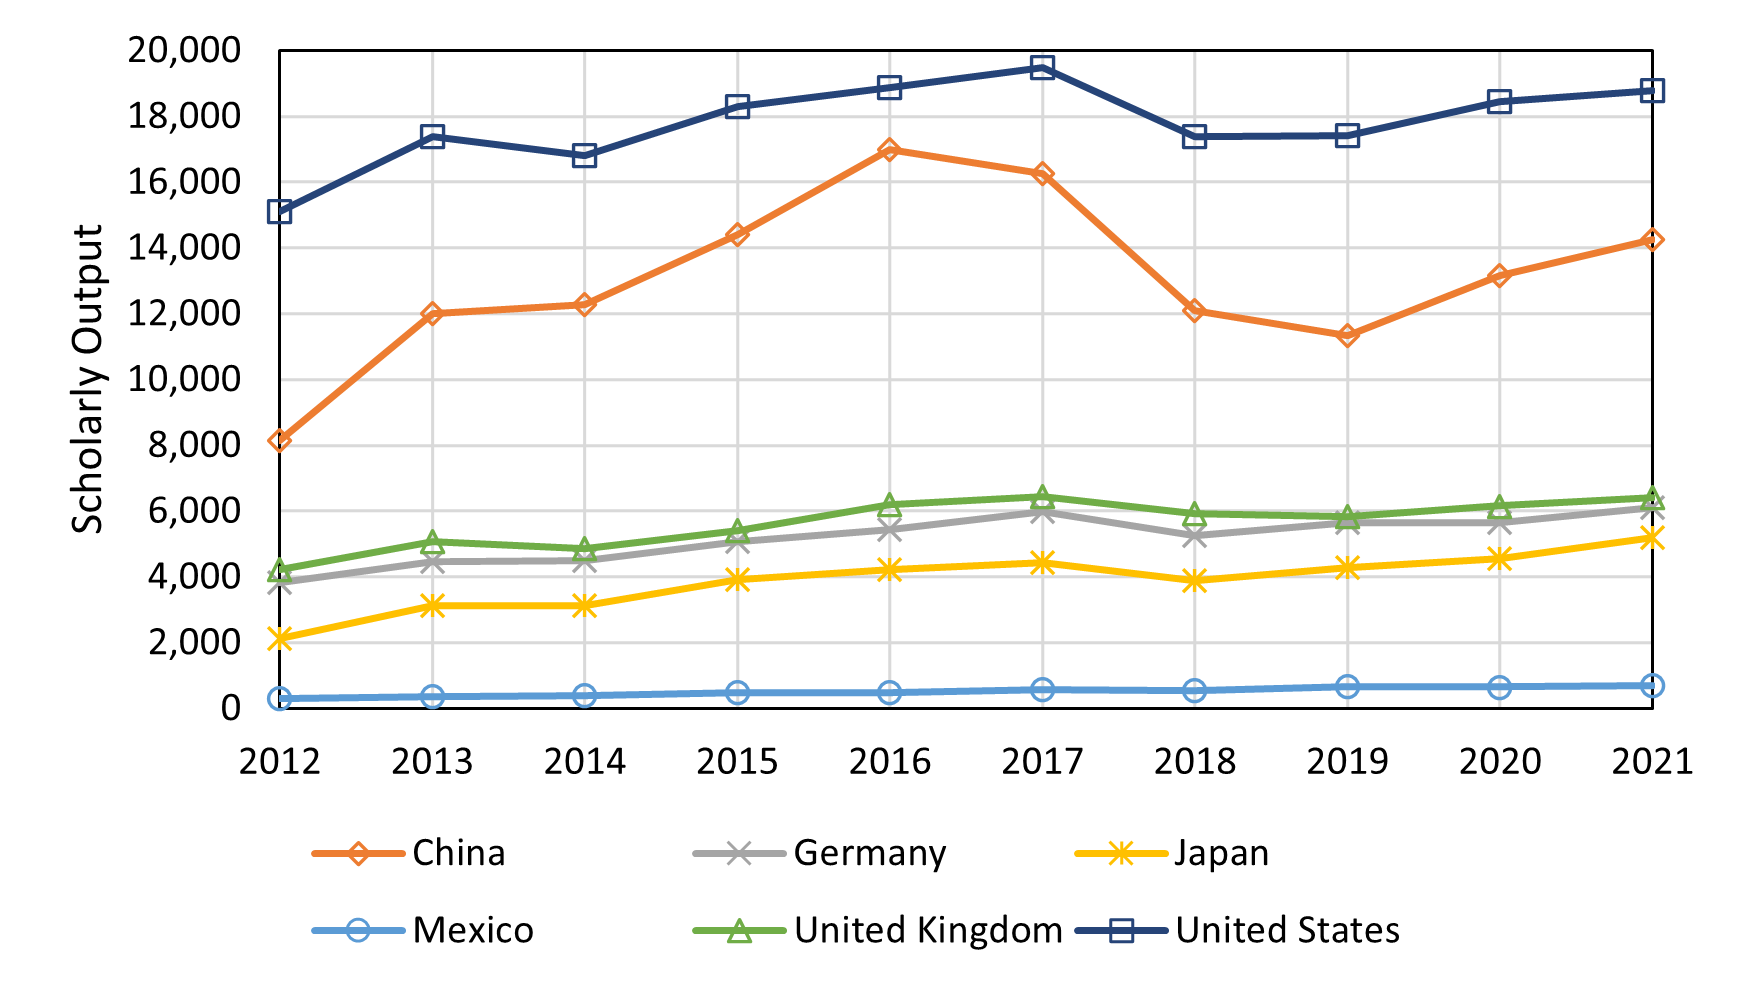
\includegraphics[width = 8 cm]{CountriesData.png}
    \caption{Time series of the top article publishing countries in the last decade excluding 2022 compared with the Mexico curve, from SciVal 2022~\cite{Scival2022} data retrieved on October 24 of 2022}
    \label{fig:CountriesData}
\end{figure}

The citation count throughout the last decade displays a similar order in ranking level; the only difference can be seen with the United Kingdom in 2012, which has around 100,000 more citations than China. However, the same ranking order is shown in Figure~\ref{fig:CountriesData}, which prevails in the following years of the citations series. All the countries with no exceptions have had more significant numbers of citations in the past; this phenomenon is expected since citations accumulate over time as it increases when new publications come out over time. The United States in 2012 had an advantage of almost 1 million sources concerning China. Although, that changed drastically by 2021, with a small gap of less than 100,000 citations. This fall has prevailed constantly through the last decade. The counts remain more constant for the United Kingdom, Germany, and Japan; however, with time, these values will experience further adjustments as new articles with more citations are published. Again, Mexico shows a dampening curve compared with the top countries, which was an expected behavior after analyzing Figure~\ref{fig:CountriesData}. The time series can be observed in  Figure~\ref{fig:CountriesCitations}, where the overall number of citations classified by country with the top 5 countries is compared with the corresponding sources for Mexican articles.

% Figure #2
\begin{figure}[H]
    \centering
    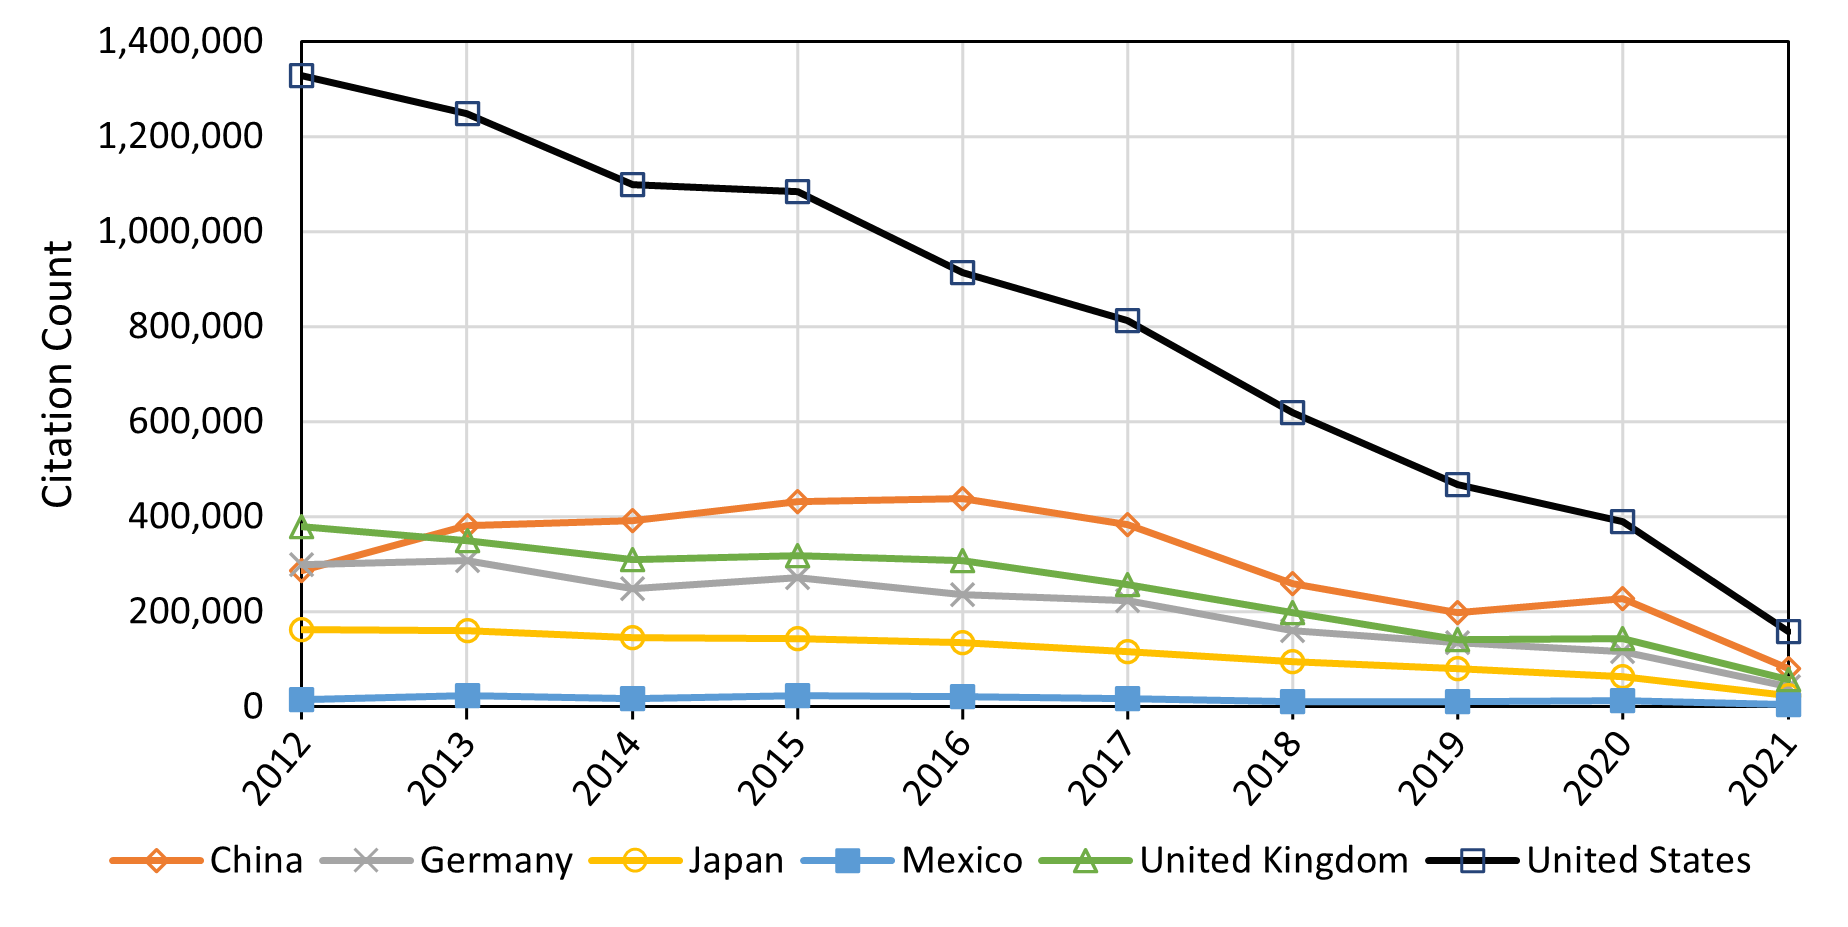
\includegraphics[width = 8 cm]{CountriesCitations.png}
    \caption{Time series of the top cited articles from the selected countries in the last decade excluding 2022 compared with the Mexico curve, from SciVal 2022~\cite{Scival2022} data retrieved on October 24 of 2022}
    \label{fig:CountriesCitations}
\end{figure}

According to the performed search, data suggest that the most popular research topics from 2012 to 2021 are the following in order of appearance, not of importance: MicroRNA, Cosmos, Cosmic Ray, Tellurium Derivative, COVID-19, Gene Regulatory Network, Elementary Particle, Biological Evolution, Hadron, and High Energy Physics. Throughout time microRNA constantly lead as one of the most popular research topics, with Biological Evolution in a less degree of popularity but with a constant tendency. Cosmic Rays and Cosmos, in general, display a repetitive pattern of falls and ascents that exceeded the scholarly output once in 2019. The rest of the topics remain in the 0-500 publications range. The fast rise of COVID-19 popularity is of particular interest starting in 2019 and staying in exponential growth for the following years, with a scholarly output of 4,500 in 2021. This data is displayed graphically in Figure~\ref{fig:Multi2} with the overall number of multidisciplinary articles from 2012 to 2021 classified by topic, where the top 10 relevant issues are compared.

% Figure #3
\begin{figure}[H]
    \centering
    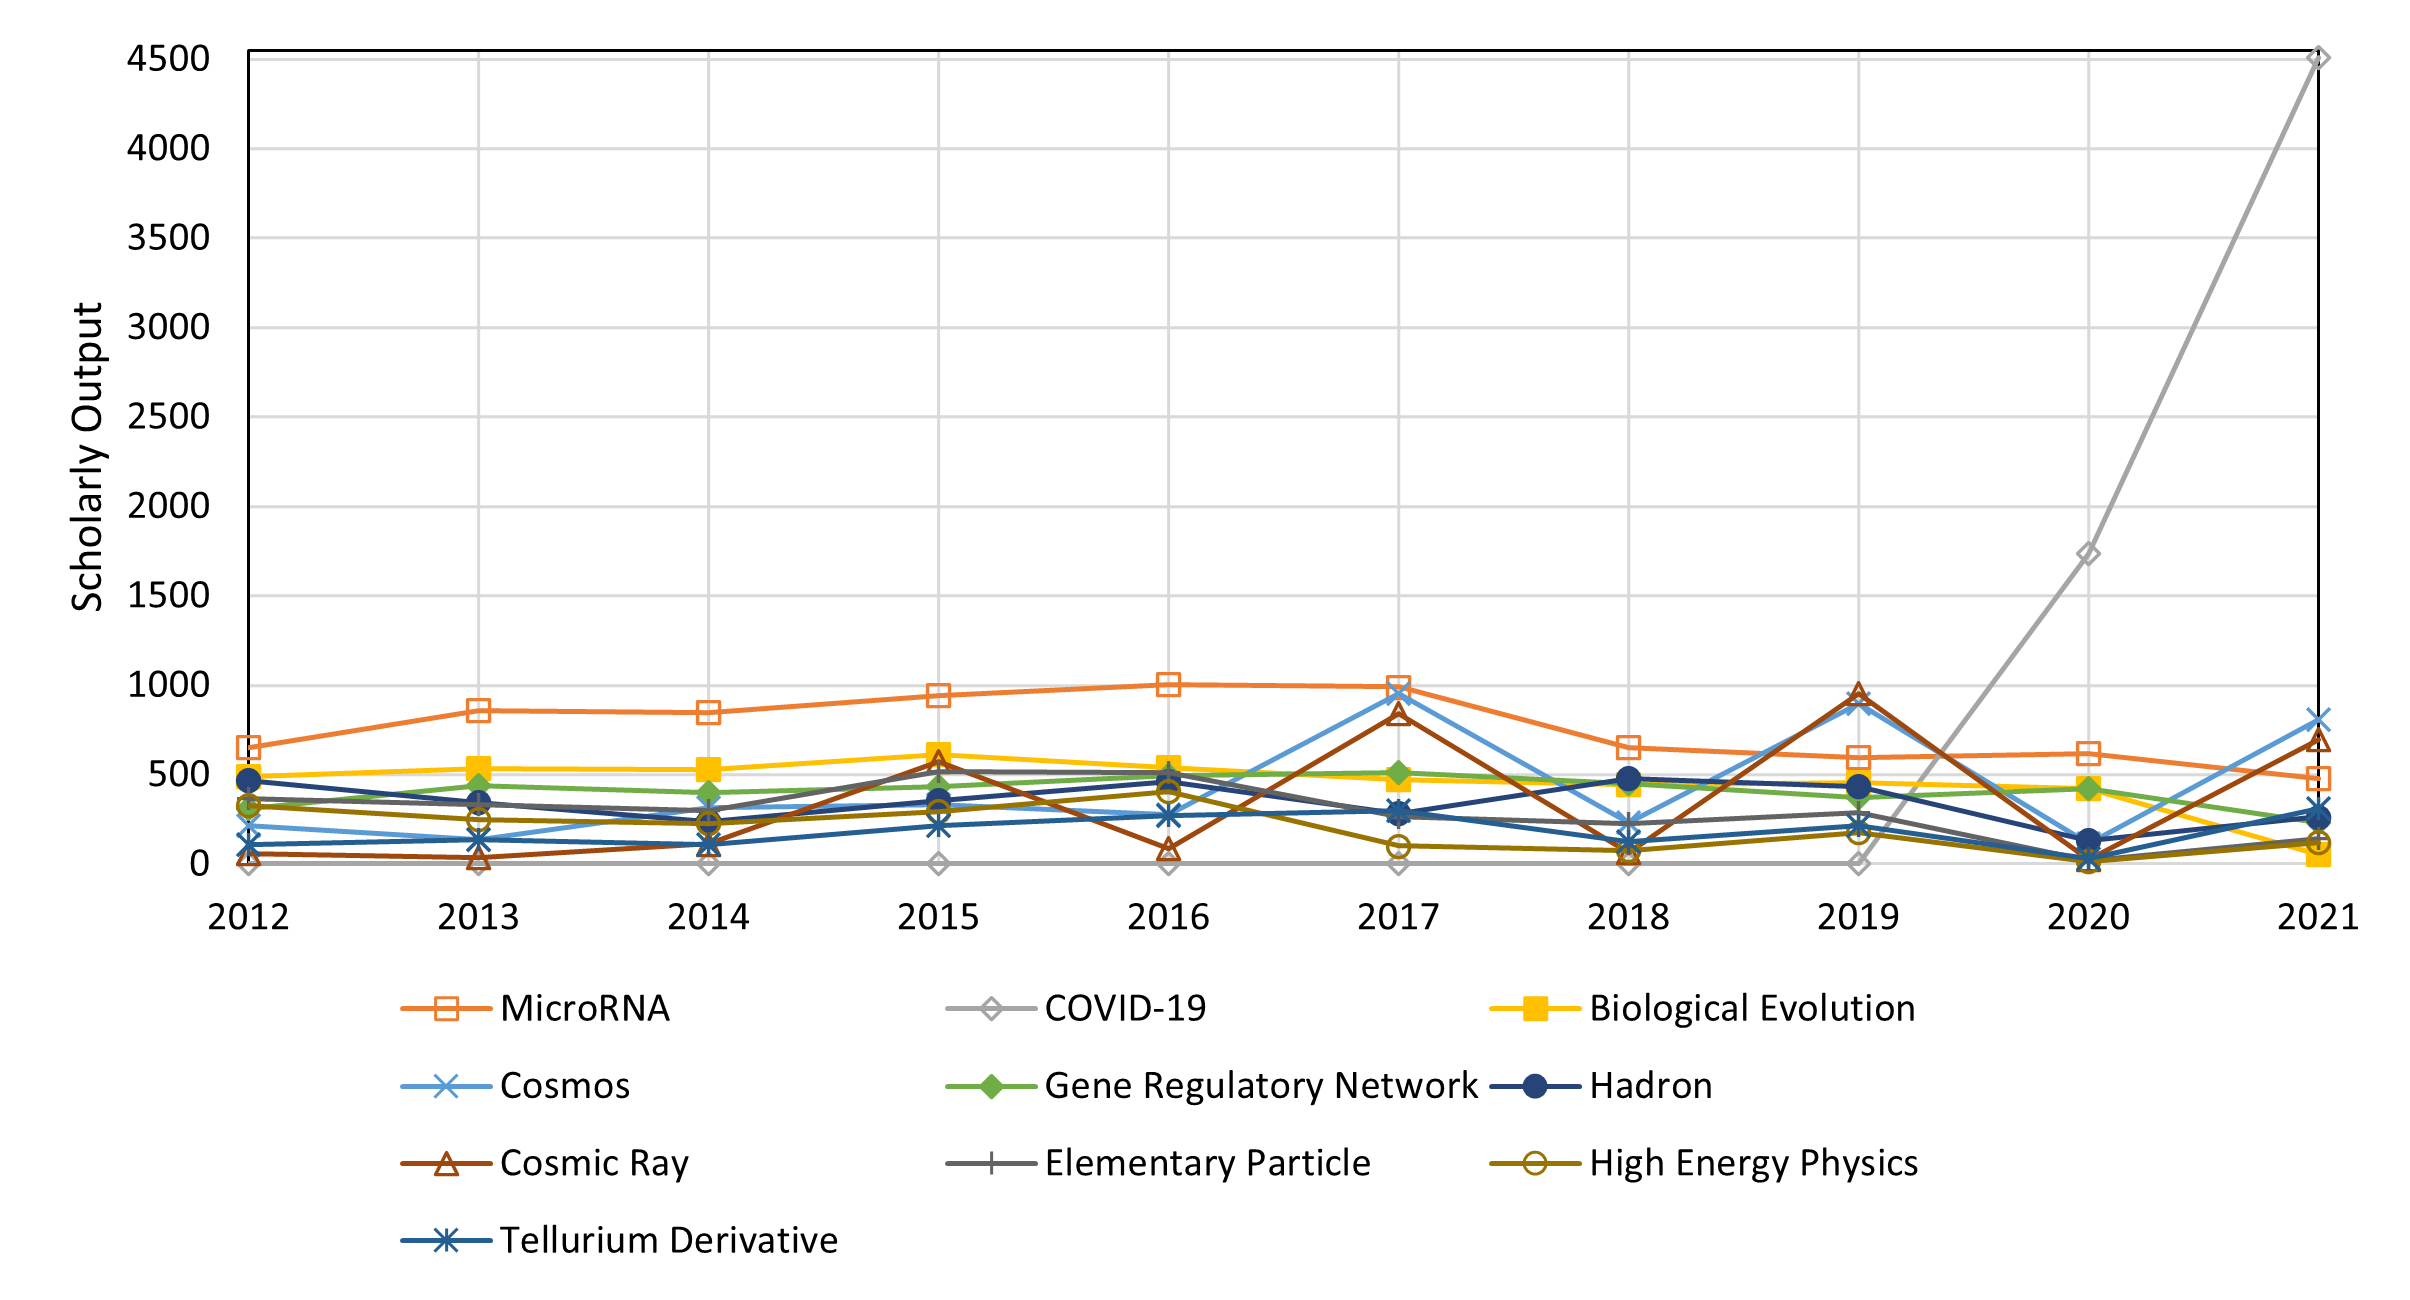
\includegraphics[width = 9 cm]{Multi2.png}
    \caption{Time series of the most popular research topics indicated by the publications number of the selected countries in the last decade excluding 2022, from SciVal 2022~\cite{Scival2022} data retrieved on October 24 of 2022}
    \label{fig:Multi2}
\end{figure}

Following the observations in Figure~\ref{fig:Multi2}~\cite{Scival2022}, the data is analyzed with a particular focus on the years range of 2019 to 2022. The published articles' keywords for the studied countries are extended in a word cloud of publications from 2019 to 2021 in Figure~\ref{fig:Multi2}~\cite{Scival2022}. Some of the most essential mentioned topics are COVID-19, Severe Acute Respiratory Syndrome, Intestine Flora, Vaccine, Neutrinos, Cosmic Ray, Meta-Analysis, MicroRNA, Cell Component, and Deep Learning, among other terms that are present in this map of words. All of these are expected after the analyzed data in Figure~\ref{fig:Multi2} since many of the keyword terms match with the most popular topics in published articles throughout 2019 to 2021

% Figure #4
\begin{figure}[H]
    \centering
    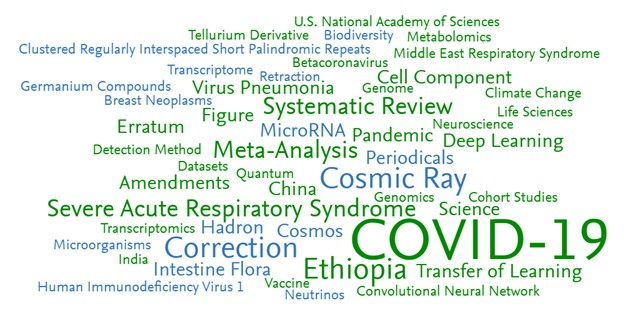
\includegraphics[width = 8 cm]{Keywords.jpg}
    \caption{Word cloud of the top published articles keywords from the United States, China, United Kingdom, Germany, Japan, and Mexico, the bigger the size, the larger the mentioning of that specific keyword, observations retrieved from SciVal 2022~\cite{Scival2022} on October 24 of 2022}
    \label{fig:Keywords}
\end{figure}

Is possible to observe in Figure~\ref{fig:Multi}~\cite{Scival2022} the overall number of multidisciplinary articles from 2019 to 2022 classified by topic, this time 2022 was not excluded from observing the whole tendency where the top 10 relevant issues are compared. Again COVID-19, along with the term pandemic and Severe Acute Respiratory Syndrome Coronavirus 2, stand for their popularity. As the scholarly output keeps increasing, the last maximum is 2021, with 4,500 publications. 2022 there is a fall since three months of the current year are missing, so it is an expected outcome. It is also quite possible that this number will keep rising until the last days of 2022. The scholarly output remained under the 0-1,500 published articles limits for the other research topics from 2019 to October 2022.

% Figure #5
\begin{figure}[H]
    \centering
    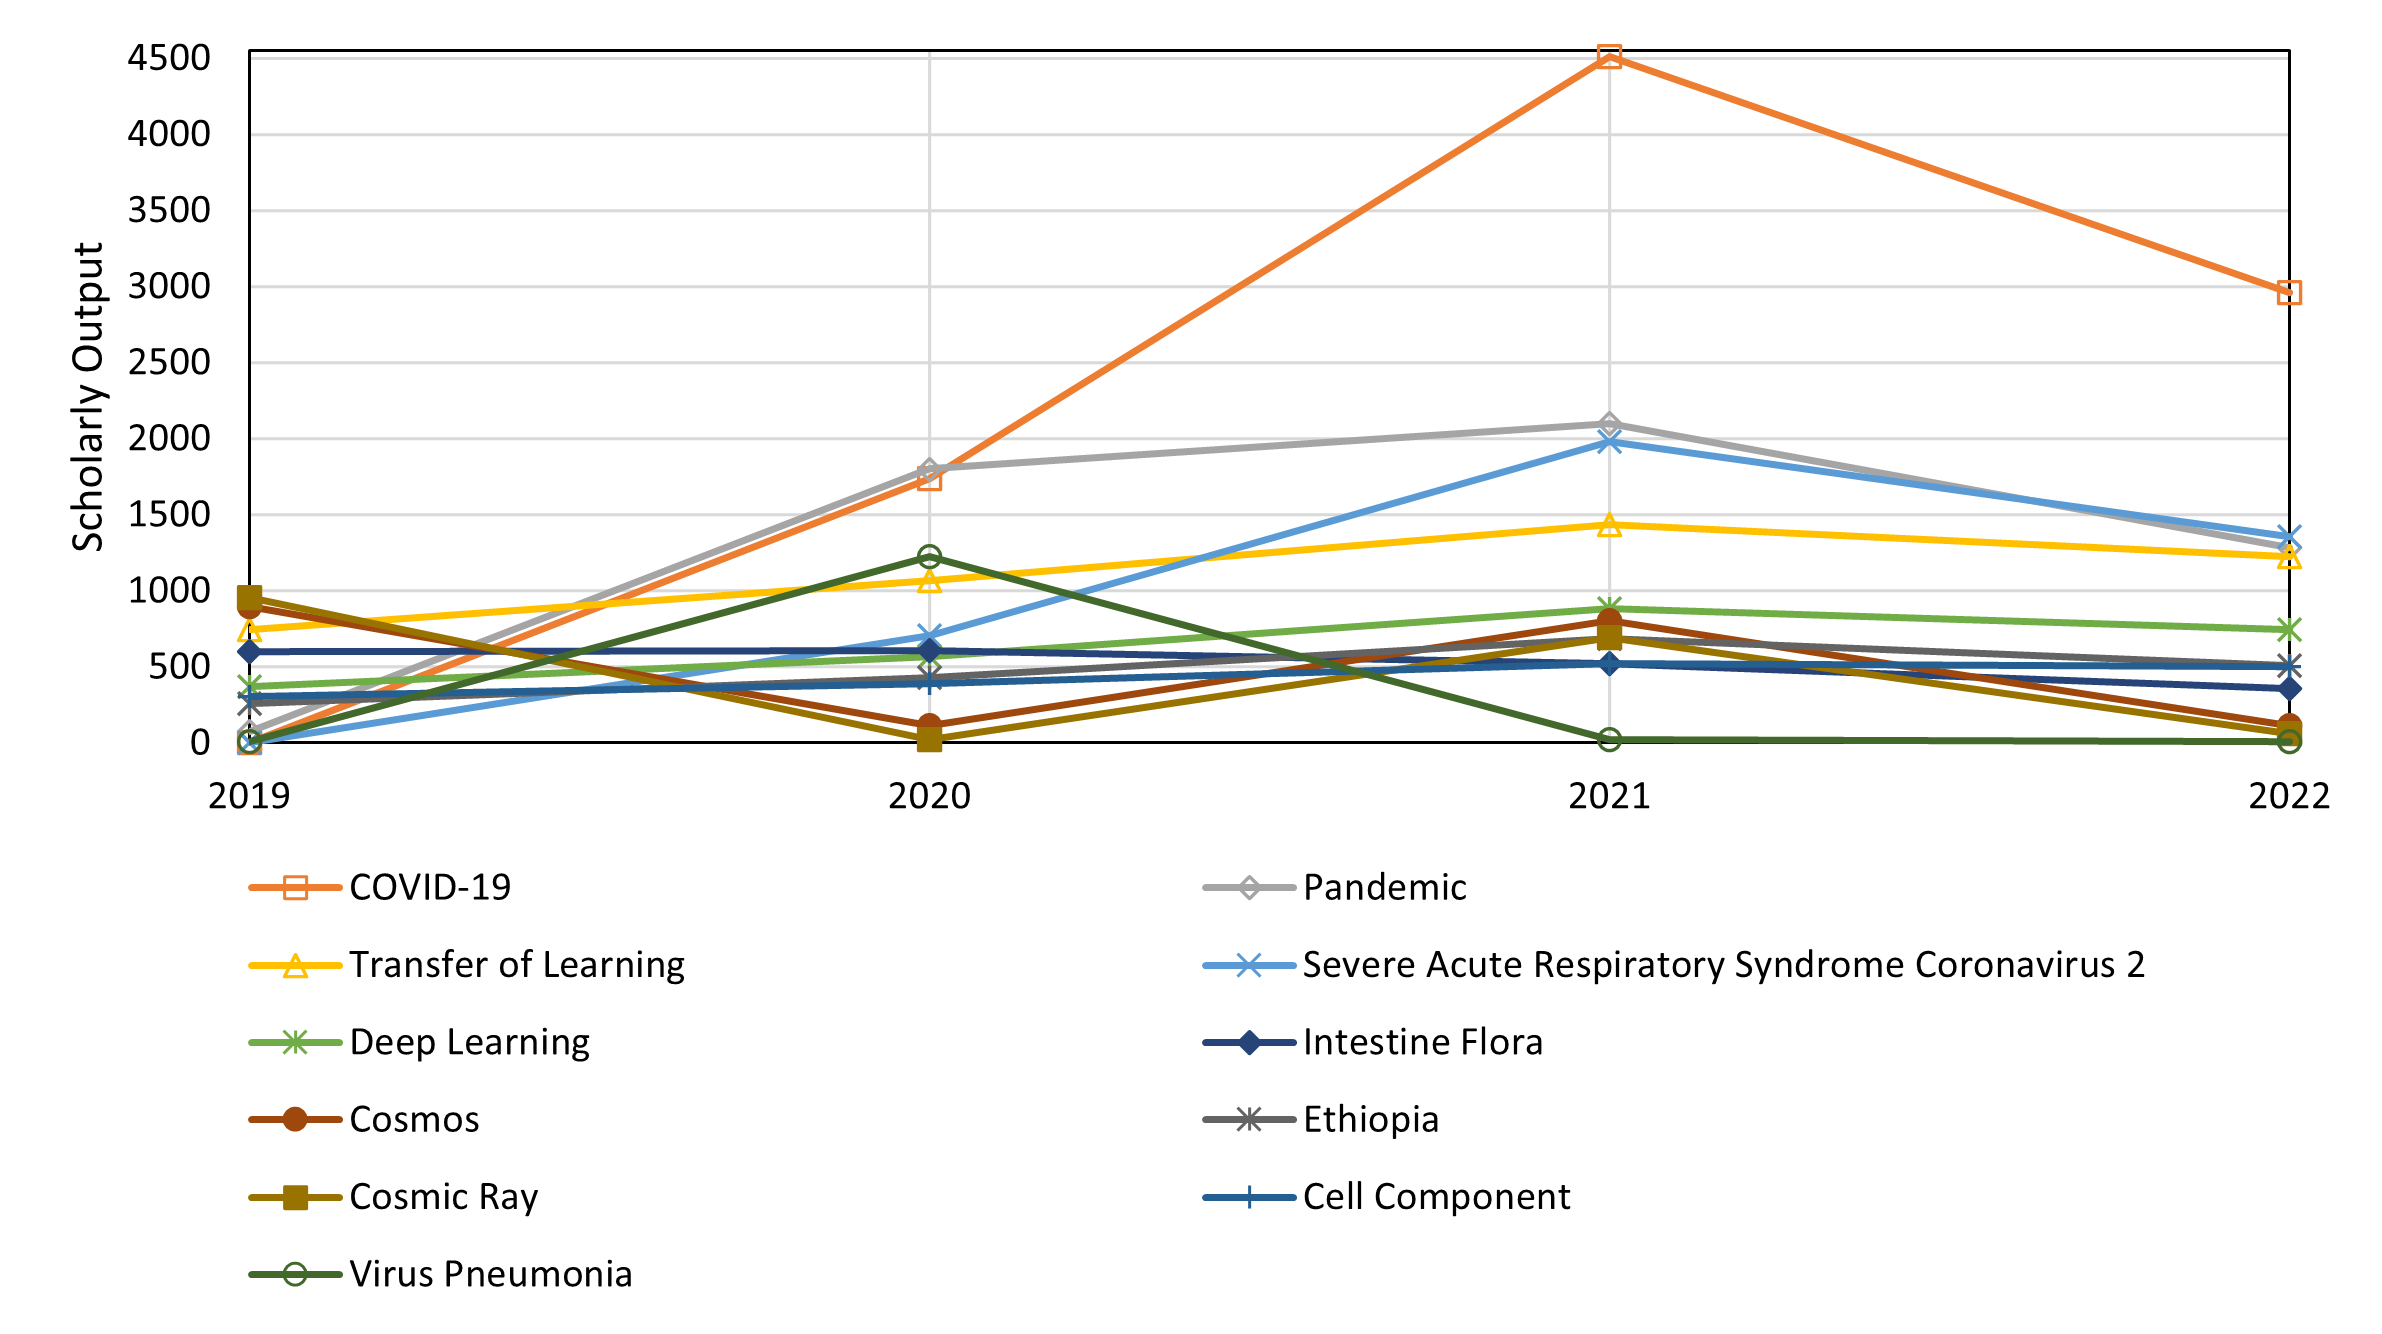
\includegraphics[width = 9 cm]{Multi.png}
    \caption{Time series of the top 10 published article topics from the United States, China, United Kingdom, Germany, Japan, and Mexico starting at 2019 to 2022, from SciVal 2022~\cite{Scival2022} data retrieved on October 24 of 2022}
    \label{fig:Multi}
\end{figure}

In the same way, since the last decade, the Chinese Academy of Sciences has been the number one publishing articles university, the 2nd is Harvard University, and both are on the rise of new coming publications. National Institutes of Health, Shangai Jiao Tong University, Tokyo University, Oxford, MIT, Peking University, Stanford, and College London are among the top ten and publish around 300-800 publications annually. These universities have tight gaps in between, so besides Shangai Jia Tong University's broad fluctuations, there is no outstanding behavior between them. The Instituto Tecnológico y de Estudios Superiores de Monterrey (ITESM) stands around 400 articles, far from the top 10 universities. However, the scholarly has been increasing in recent years. The time series can be observed in Figure~\ref{fig:Universities}, where the overall Scholarly Output is classified as top universities compared with the ITESM.

% Figure #6
\begin{figure}[H]
    \centering
    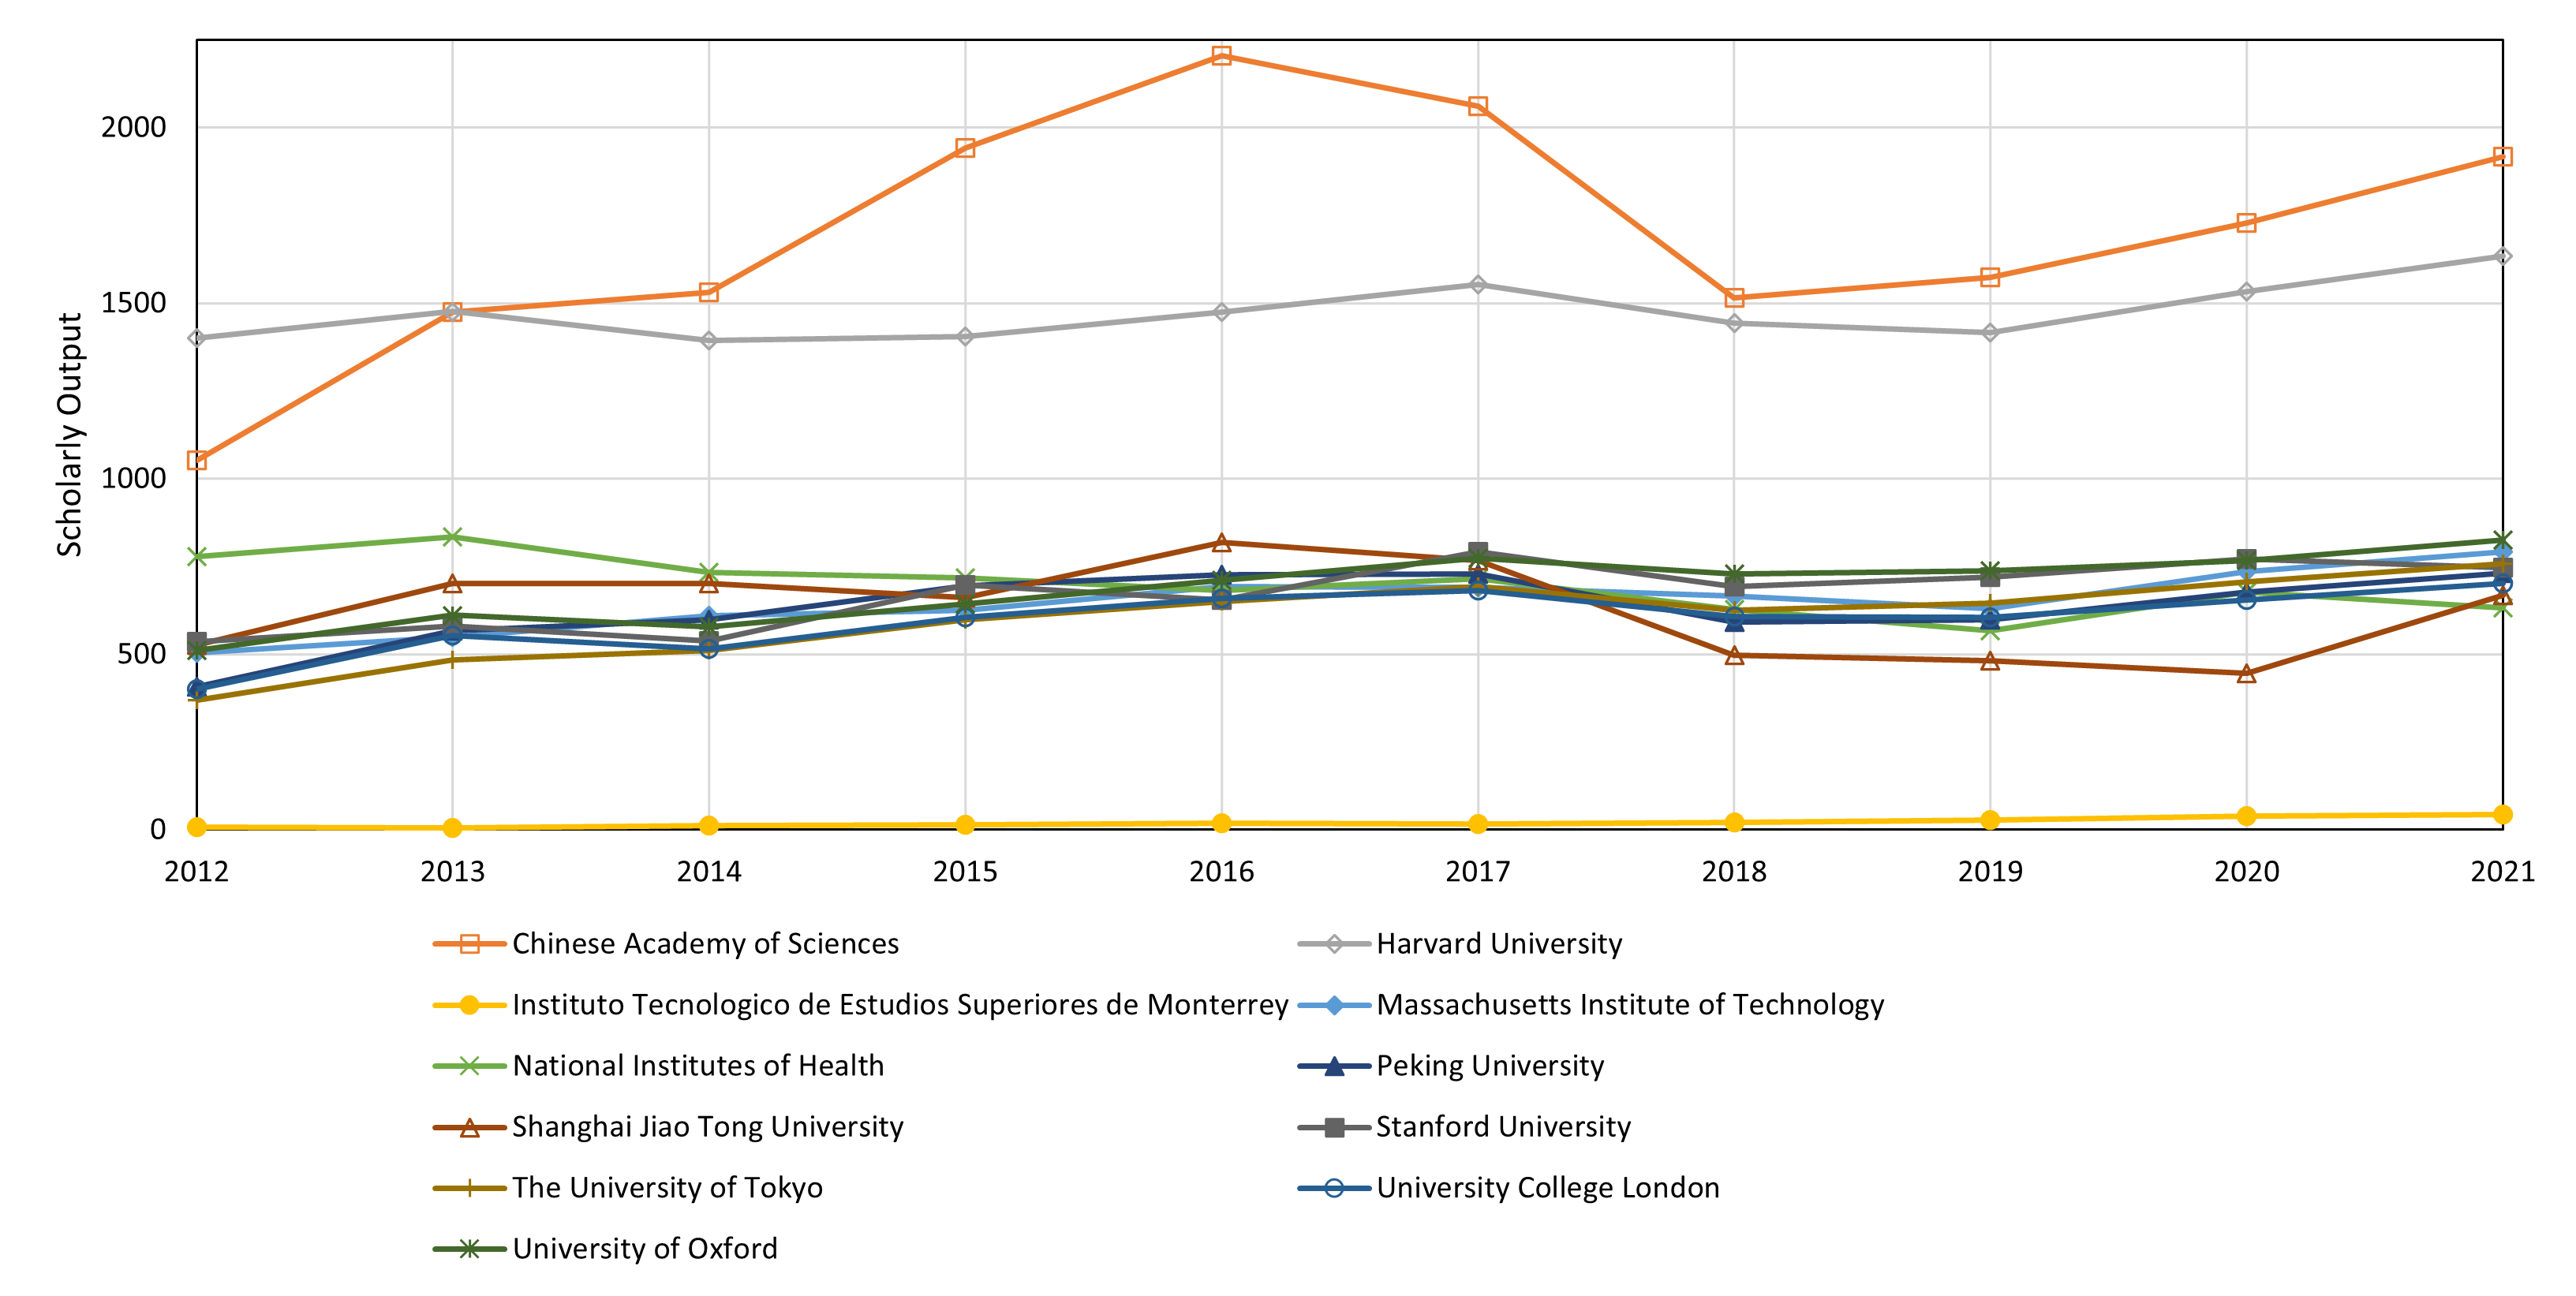
\includegraphics[width = 9 cm]{Universities.png}
    \caption{Time series of the top publishing articles universities in the last decade excluding 2022 compared with the Instituto Tecnológico y de Estudios Superiores de Monterrey curve, from SciVal 2022~\cite{Scival2022} data retrieved on October 24 of 2022}
    \label{fig:Universities}
\end{figure}

As citation depends to some extent on the scholarly output expressed in published articles, Harvard University, MIT, and the Chinese Academy of Sciences are on top, with values ranging from 60,000 citations to 240,000 citations. Stanford University, the National Institutes of Health, Oxford University, University College London, The University of Tokyo, Peking University, and Shangai Jiao Tong University are among the top 10 institutions cited in released articles. On this plot is harder to appreciate a visible growth in the last years for the Tecnológico de Monterrey. However, this was expected since it is a young research institution that shifted from a teaching to a research university in the last 20 years. The time series can be observed in Figure~\ref{fig: Universities2}, where the overall citation count is classified with the top universities compared with the ITESM.

% Figure #7
\begin{figure}[H]
    \centering
    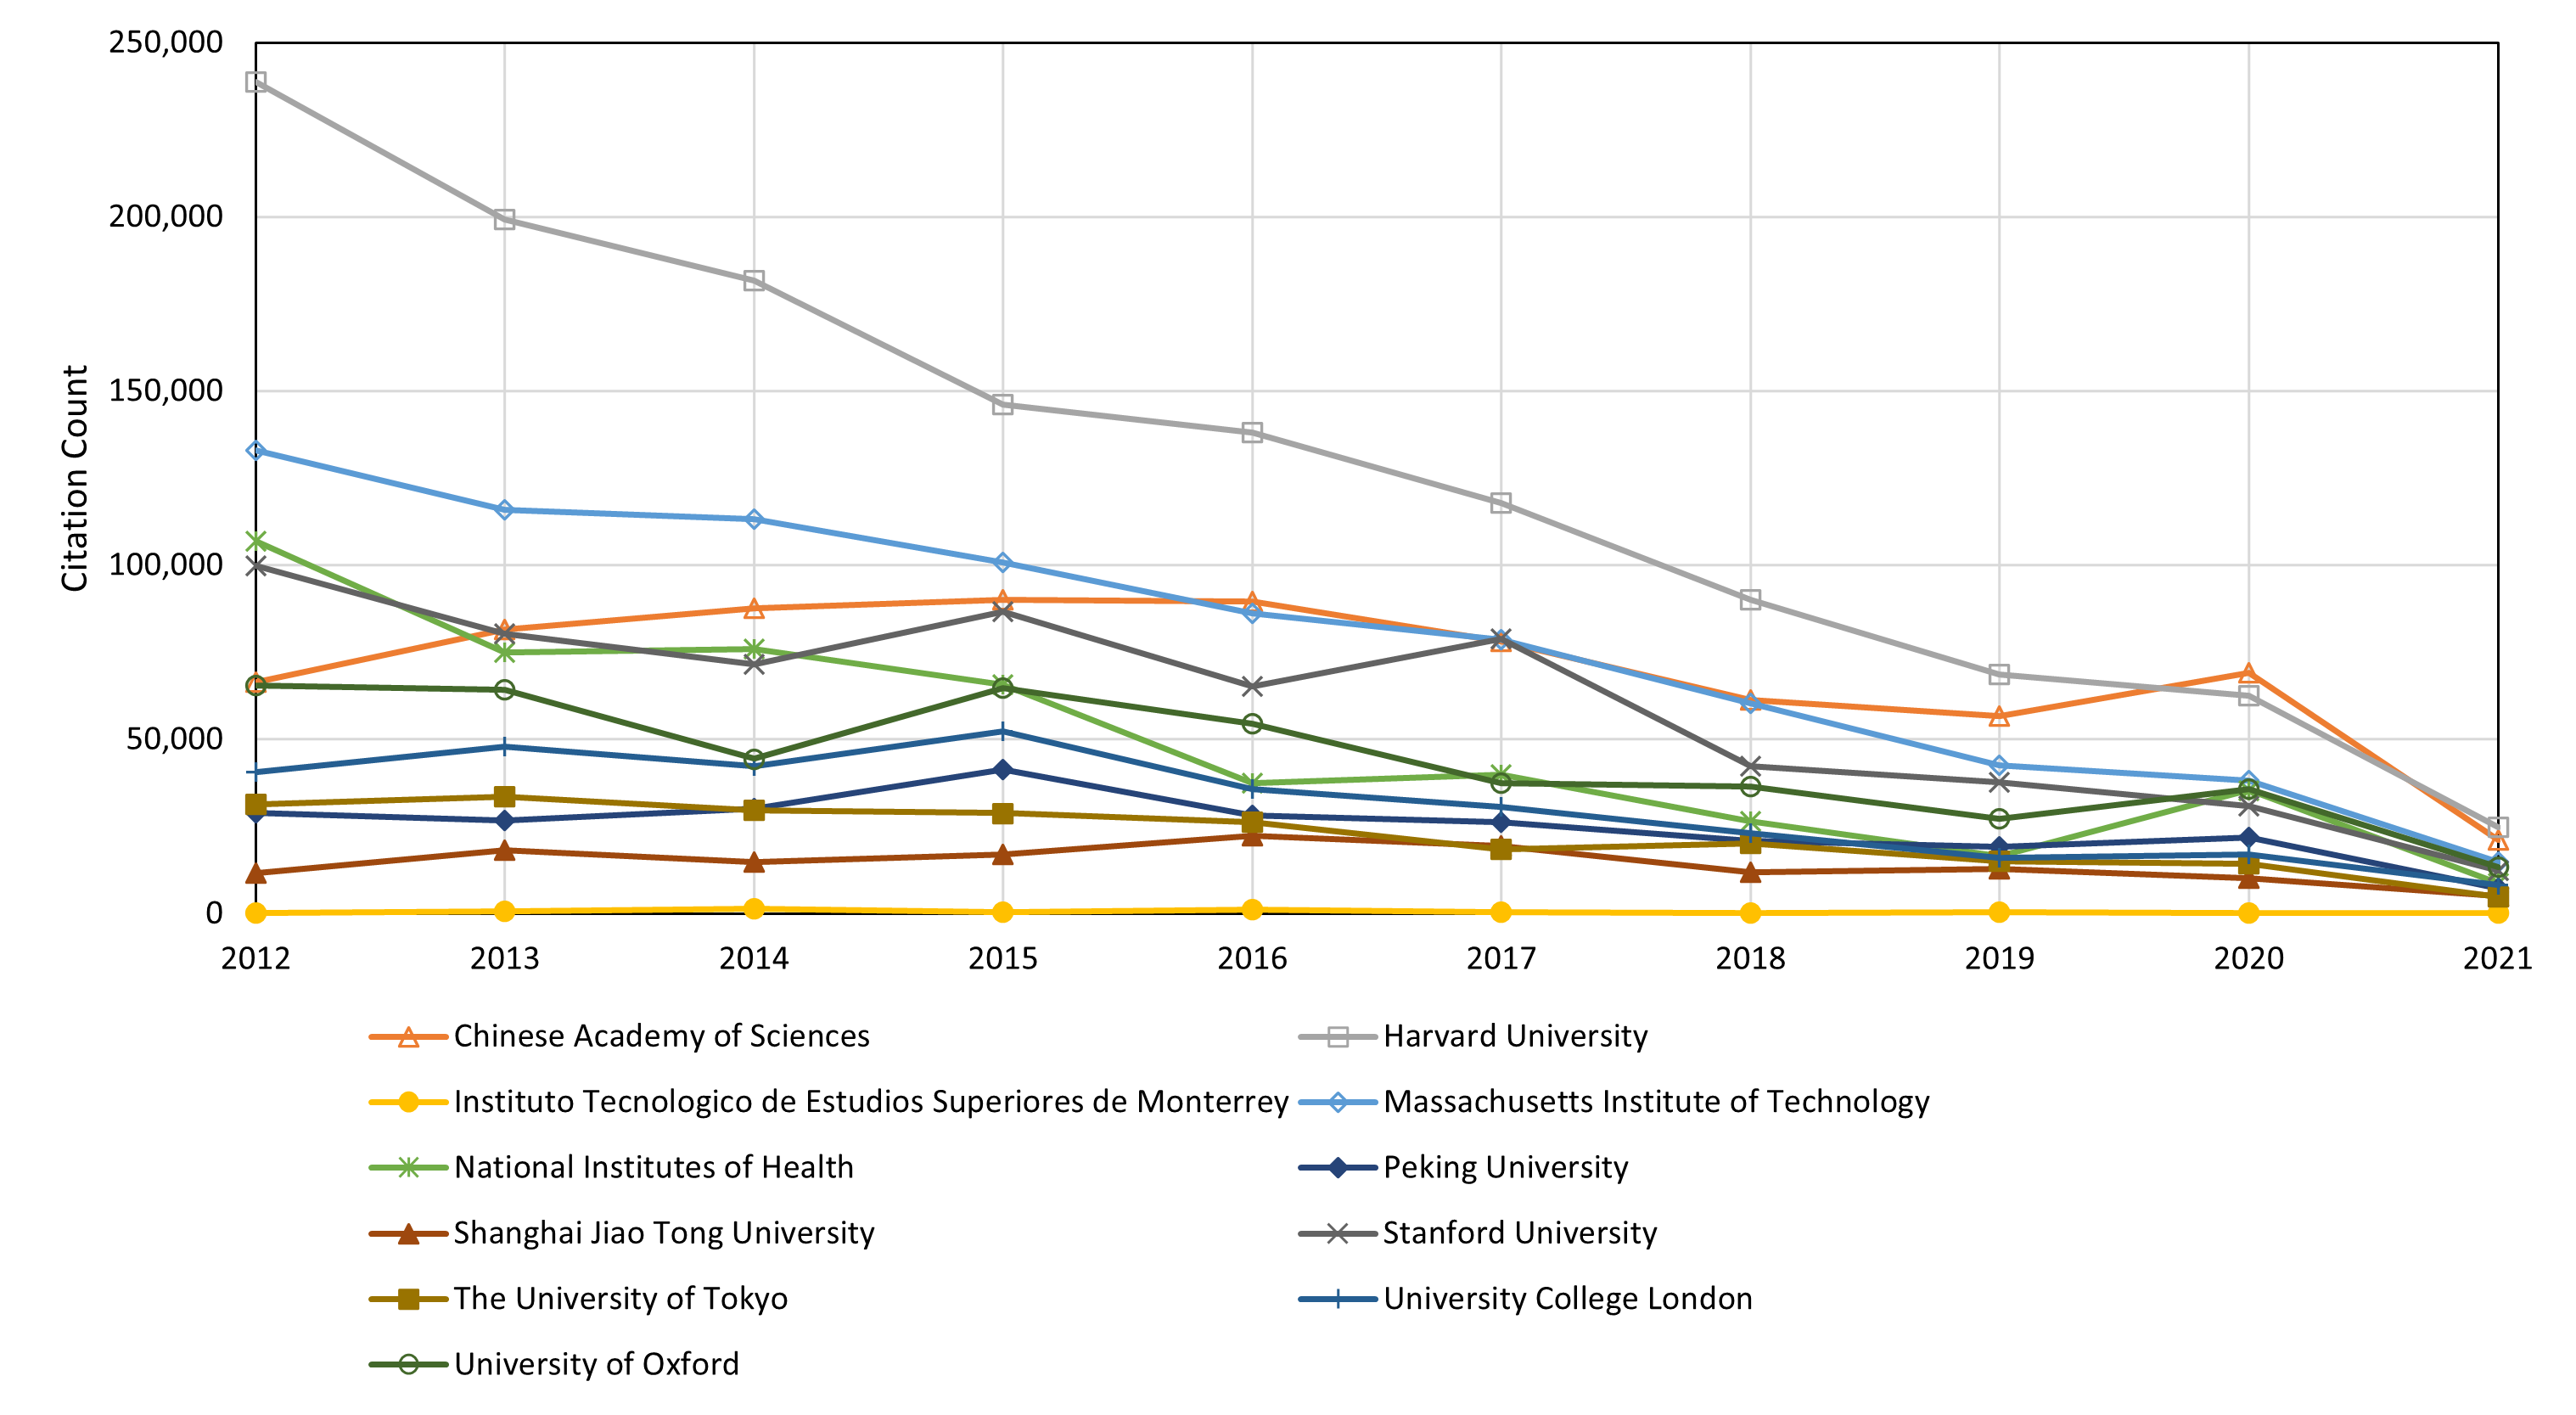
\includegraphics[width = 8 cm]{Universities2.png}
    \caption{Time series of the top cited articles universities in the last decade excluding 2022 compared with the Instituto Tecnológico y de Estudios Superiores de Monterrey curve, from SciVal 2022~\cite{Scival2022} data retrieved on October 24 of 2022}
    \label{fig:Universities2}
\end{figure}
%---------------------------------------------------------------------------------------------------------------

%---------------------------------------------------------------------------------------------------------------
\section{Discussion}
\label{sec:Discussion}

As reported in figures \ref{fig:Multi2} and \ref{fig:Multi}, multidisciplinary research has topics about biology, computer science, physics, etc. But by the end of 2019, this area's primary focus is Covid-19. A pandemic is now a historical event that demonstrates by this results the capacity of the different regions to work together and with different approaches to tackle the significant problem caused by this disease. 
Particularly in the case of the universities of the United States, an excellent collaboration among different research areas may be the main factor behind the outstanding number of articles and cites regarding multidisciplinary research. It would also be interesting to analyze the relationship between interdisciplinary research by countries and the response of those countries against the pandemic to get insights into the impact of this type of research on big problems. It would also be interesting to keep track of the different areas that conform to this multidisciplinary research, compare them several years after COVID-19, and evaluate if this event changed this type of research.
%---------------------------------------------------------------------------------------------------------------

%---------------------------------------------------------------------------------------------------------------
\section{Conclusion}
\label{sec:Conclusion}
In this article, the analyzed subject was multidisciplinary research between the five countries, with most published articles viewed from the Mexico scenario. From the results, it is clear that the leading countries that contribute and have more citations in this area are the USA and China; groups of 3 countries also perform well. However, Mexico is far from these countries. It is also true that the results show a slight increase in articles and citations for both Mexico and ITESM. 

Considering these results, we can learn that it has progressed over the past years. Still, it is essential to focus on helping and promoting multidisciplinary work among different topics for a more significant change. Another important observation from the results is that in the last couple of years, the most popular issues of published articles have changed drastically due to the COVID-19 pandemic. The research interest shifted to a more multidisciplinary approach, which in the end, is an exciting indicator of how effective it can be to unite different disciplines to tackle an urgent problem.

For further studies, it is important to delimit the essential topics in multidisciplinary research; some may become formal areas that can be analyzed more specifically. Time series analysis and forecasting of the country's productivity, both sites have the opportunity to be studied in detail to find hidden patterns in data that can be analyzed to understand the scenario for each country and its tendencies for the following years.
%---------------------------------------------------------------------------------------------------------------
\section{Research Profiles}
The generation of the profile of Farid Jácome for Google Scholar presented some complications since it requires a published document to create the account. However, other reports could be generated.

\begin{figure}[H]
    \centering
    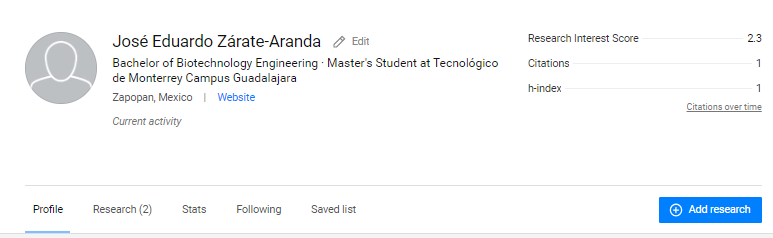
\includegraphics[width = 8 cm]{JEDZA1.png}
    \caption{José Eduardo Zárate-Aranda research profile in Researchgate}
    \label{fig:JEDZA1}
\end{figure}

\begin{figure}[H]
    \centering
    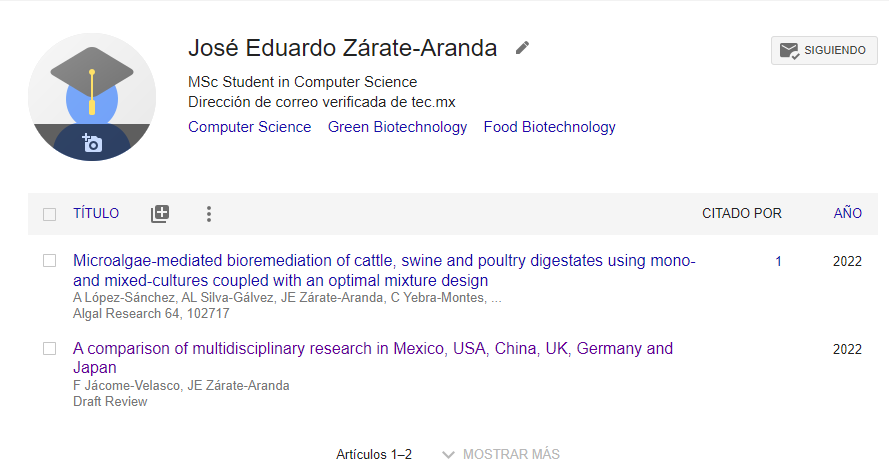
\includegraphics[width = 8 cm]{JEDZA2.png}
    \caption{José Eduardo Zárate-Aranda research profile in Google Scholar}
    \label{fig:JEDZA2}
\end{figure}

\begin{figure}[H]
    \centering
    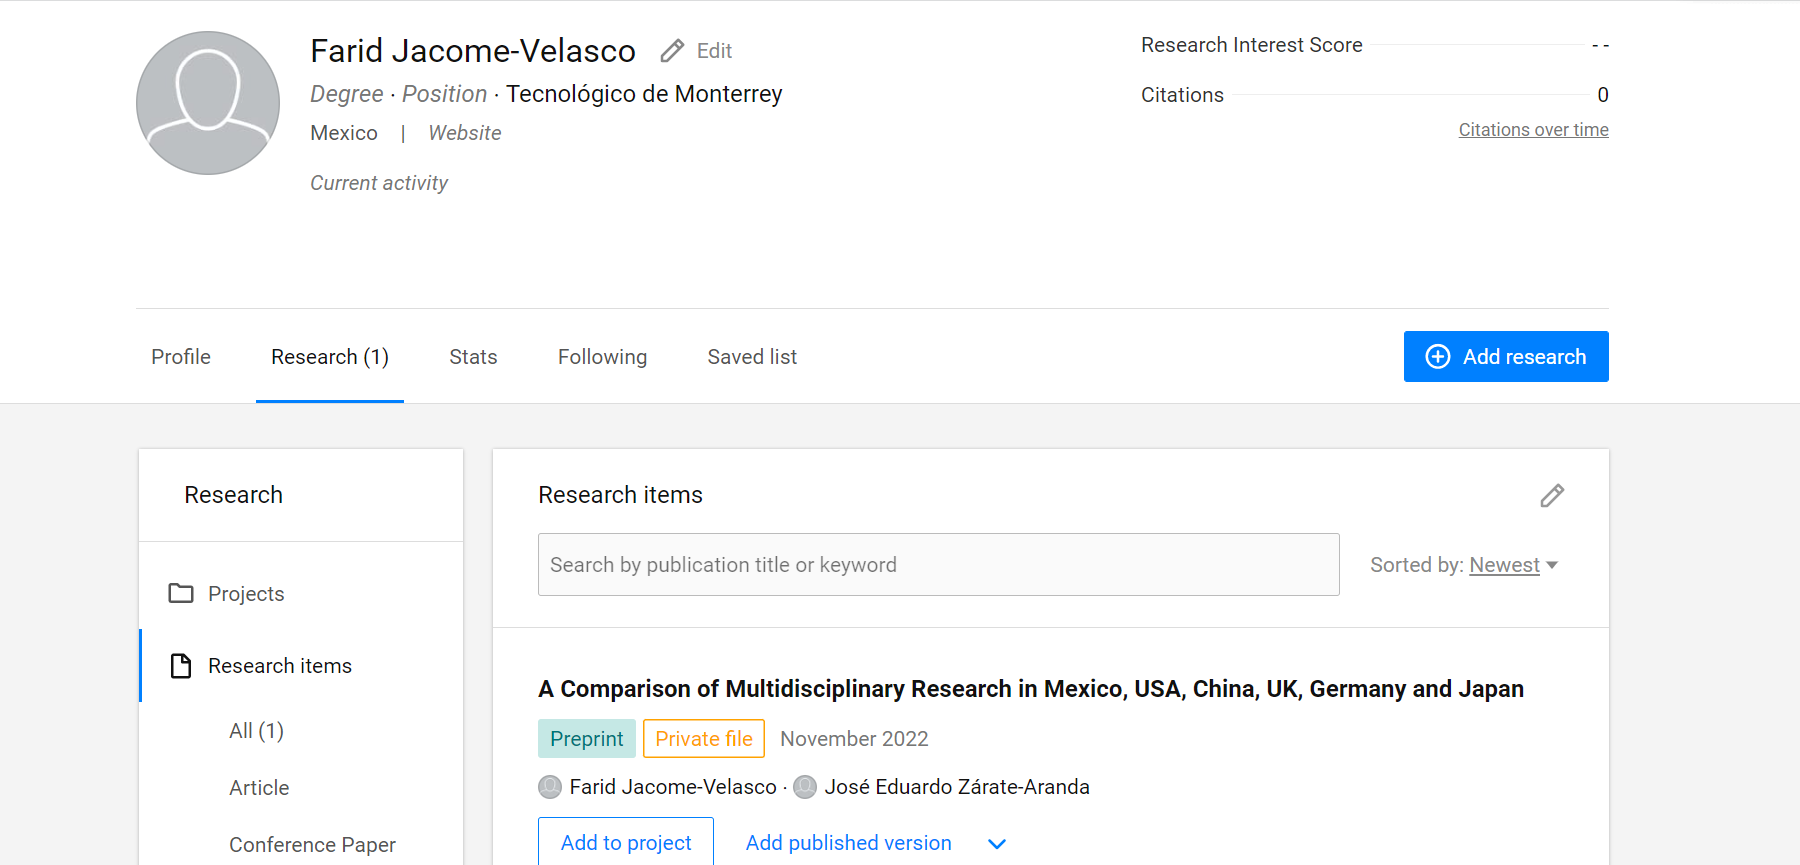
\includegraphics[width = 8 cm]{Farid1.png}
    \caption{Farid Jácome Velasco research profile in Researchgate}
    \label{fig:Farid1}
\end{figure}

%---------------------------------------------------------------------------------------------------------------
\bibliographystyle{plain}
\bibliography{Scival_Review_References.bib}
%---------------------------------------------------------------------------------------------------------------
\end{document}